\documentclass[a4paper,oneside]{book}
\usepackage{anysize}
\usepackage{lastpage}
\usepackage{fancyhdr}
\usepackage{polyglossia}
\setdefaultlanguage[variant=uk]{english}
\usepackage{fontspec}
\usepackage{color}
\definecolor{bkg}{rgb}{0.9,0.9,0.9}
\definecolor{cmt}{rgb}{0.0,0.6,0.0}
\definecolor{boxbkg}{rgb}{0.9,0.95,1.0}
\usepackage{fancybox}
\usepackage{mdframed}
\usepackage{listings}
\defaultfontfeatures{Ligatures=TeX}
\usepackage{graphicx}
\graphicspath{{./logo/}{./img/}}
\usepackage[x11names]{xcolor}
\usepackage[colorlinks=true]{hyperref}
\usepackage{framed}
\usepackage{float}
\usepackage{wrapfig}
\restylefloat{figure}
\usepackage{makeidx}
\usepackage{listings}
\usepackage{amsmath}
\usepackage{realboxes}

\newtoggle{InString}{}% Keep track of if we are within a string
\togglefalse{InString}% Assume not initally in string

\definecolor{light-gray}{gray}{0.95}

\lstset{
    backgroundcolor=\color{bkg},
    basicstyle=\small\ttfamily,
    breaklines=true,
    columns=fullflexible,
    numbers=left,
    numberstyle=\tiny,
    keywordstyle=\color{blue},
    commentstyle=\color{cmt},
    stepnumber=5,
    captionpos=b,
}
\lstdefinelanguage{json}{
    string=[s]{"}{"},
    showstringspaces=false,
    % stringstyle=\color{black},
    morecomment=[s][\color{purple}\ttfamily]{\ \ \"}{\"},
    morecomment=[s][\color{black}\ttfamily]{\ \ \ \ \ \"}{\"},
    % keywords=[1]{true, false},
    % keywordstyle=[1]\color{cyan},
    columns=flexible,
    keepspaces=true,
    morecomment=[l]{//},
}
\usepackage{caption}
\usepackage{subcaption}

\marginsize{1.5cm}{1.5cm}{0.5cm}{1.7cm}
\pagestyle{plain}
\setmainfont{Reporter}
\makeindex

\begin{document}
\begin{figure}[h]
  \includegraphics[width=\textwidth]{doc_head.jpg}
\end{figure}

\parindent=0pt
\parskip=0.25cm

\begin{center}
\fontsize{20}{21}\selectfont

\textbf{SelfHelp WebApp} - Create Web Applications Serving as a Platform for Research Experiments\\
\vskip 6mm
Tutorial for version v0.9.10
\vskip 6mm

\fontsize{13}{14}\selectfont
Simon Maurer - \texttt{simon.maurer@humdek.unibe.ch}\\
\today
\end{center}

\tableofcontents

%==============================================================================
\chapter{Introduction}\label{sec.intro}

This documentation refers to the TPF project \href{http://phhum-g111-nns.unibe.ch:10012/SLP/SLP-sleep_coach}{SLP-selfhelp}.
The project aims at providing a tool that allows to create a web application that serves as a platform for research experiments.
The basic concept is as follows:

Pages are organised as a collection of sections that are rendered on the page, one below the other.
Sections have different styles which define the appearance of the sections.
Depending on the style of a section, the section has different fields which define the content of the section.
The value of a field can be a simple plaintext or a collection of child sections which have their own styles and children.

Currently available styles include, but are not limited to, alert boxes, buttons, card containers, forms, media elements, tabs, lists, and support for markdown texts.

The app is designed in such a way that it can be extended with new styles or custom components without having to modify existing code.

The main purpose of this document is to provide a step-by-step tutorial of how to work with the admin section of the SelfHelp WebApp.

For an overview of existing styles and their fields refer to \href{https://selfhelp.psy.unibe.ch/demo/styles}{this demo page}\footnote{https://selfhelp.psy.unibe.ch/demo/styles}.
Instructions for configuring the web server can be found on \href{https://selfhelp.psy.unibe.ch/demo/configs}{this page}\footnote{https://selfhelp.psy.unibe.ch/demo/configs}.
For the documentation of the source code refer to \href{https://selfhelp.psy.unibe.ch/demo/doc/doxygen/html/index.html}{this doxygen page}\footnote{https://selfhelp.psy.unibe.ch/demo/doc/doxygen/html/index.html}.
Finally, \href{https://selfhelp.psy.unibe.ch/demo/extend}{this page}\footnote{https://selfhelp.psy.unibe.ch/demo/extend} provides some information about possible extension and customization options of the WebApp.

In the following it is assumed that a server is up and running and an instance of this WebApp is made available.
After a clean setup an account \texttt{admin} is activated which can be accessed with the password \texttt{admin};

%==============================================================================
\chapter{Creating a New Page}
\label{sec.new_page}
In order to crate a new page the \texttt{select} and \texttt{insert} access right of \textbf{Page Management} are required.
By default users in the group \texttt{admin} and \texttt{experimenter} are granted the mentioned access rights.

Once logged in, navigate to the \emph{Content Management System (CMS)} in the menu \emph{Admin} and click the button \emph{Create New Page} in the top left corner.

\begin{figure}[ht]
    \centering
    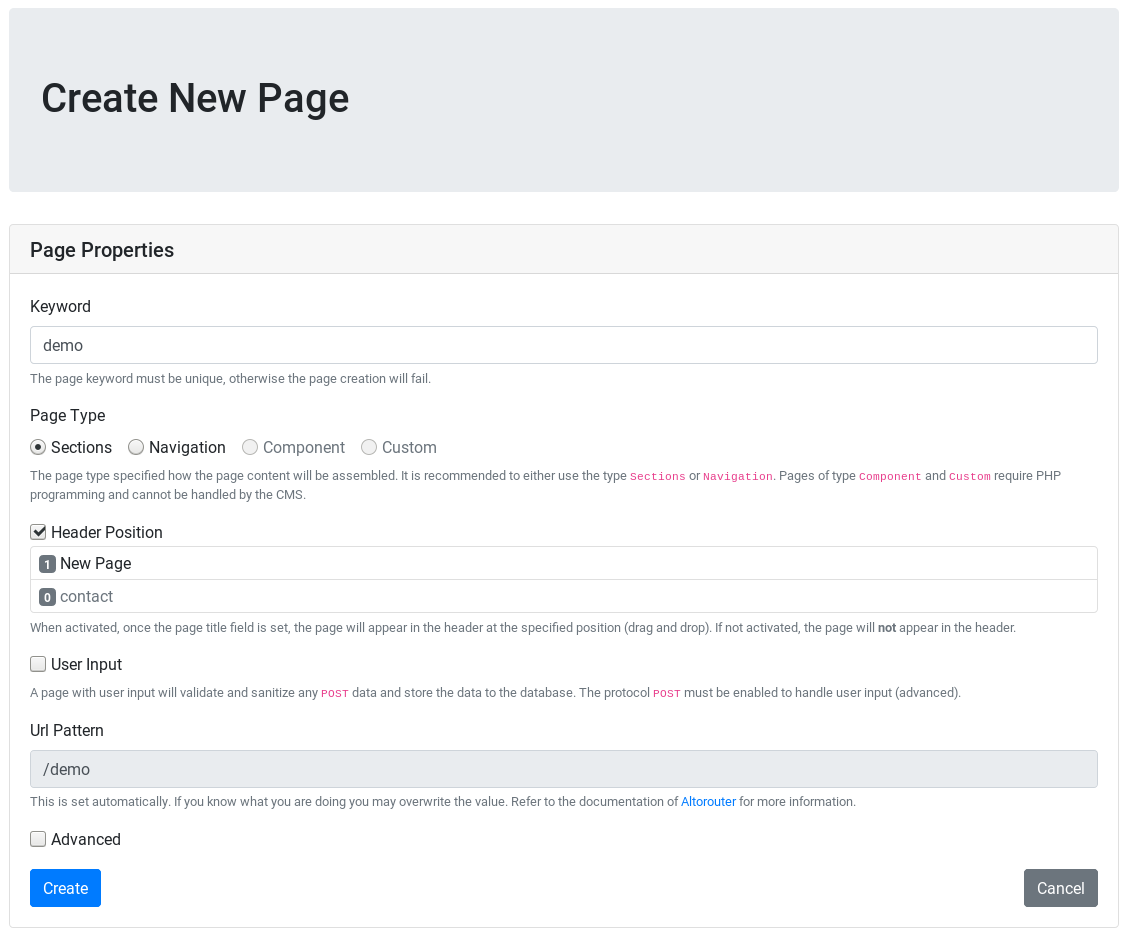
\includegraphics[width=0.95\textwidth]{create_page.png}
    \caption{The \emph{Create New Page} form.}
    \label{fig.create_page}
\end{figure}

This opens the \emph{Create New Page} form (see Figure~\ref{fig.create_page}) where properties of the new page can be entered:
\begin{description}
    \item[Keyword]
        This must be a unique name which is used to identify a page internally (e.g. \Colorbox{light-gray}{\lstinline[columns=fixed]|demo|}).
        This is also the name that will be used in the CMS when a link to this page must be shown.
        Note that this field is not visible for a user without access to the CMS (e.g. a subject).
    \item[Page Type]
        The page type specified how the page content will be assembled.
        Choose type \textbf{Sections}.
    \item[Header Position]
        Enable this field to make the page appear as a menu-point in the navigation bar of the WebApp.
        Drag and drop the item \textbf{New Page} to the location you want it to appear.
        Note that the page will only appear as a menu item once the \texttt{title} field is set (this must be done after the page creation process).
    \item[Headless Page (advanced only)]
        This allows to select whether the page will be rendered with (default) or without header and footer.
    \item[Protocol (advanced only)]
        The protocol specifies how a page is accessed.
        Do not change this.
    \item[Url Pattern (advanced only)]
        This field describes the url path of how the page will be accessible.
        By default the keyword is used.
    \item[Advanced]
        Set this flag if you wish to specify advanced options.
        This includes
        \begin{itemize}
            \item the selection of the \emph{Page Type} \textbf{Component} or \textbf{Custom}.
            \item the selection of the \emph{Protocol}.
            \item changing the \emph{Url Pattern}.
            \item changing the \emph{Headless Page} parameter.
        \end{itemize}
\end{description}

Click the button \textbf{Create} to create the page and on success the button \textbf{To the new Page} to return back to the CMS with the new page selected.

%------------------------------------------------------------------------------
\section{Add Content to the Page}
\label{sec.add_content}
In order to add content to a page the \texttt{update} access right of \textbf{Page Management} is required.
By default users in the group \texttt{admin} and \texttt{experimenter} are granted the mentioned access rights.

In a first step let's define the title of the page \Colorbox{light-gray}{\lstinline[columns=fixed]|demo|}.
The title is used as label for the menu item in the navigation bar of the WebApp and will appear in the browser tab.
To set the page title select the pen symbol in the top right corner of the \emph{Page Properties} card.
Doing so will change the card colour to yellow and provide an input field where the title can be entered.
If you just created a new page you will already be in edit mode (which is indicated by the yellow border of the \emph{Page Properties} card).
Change the field \texttt{title} (e.g. to \Colorbox{light-gray}{\lstinline[columns=fixed]|Demo|}) and click \textbf{Submit Changes} to make the change permanent.
If during the creation of the page the option \emph{Header Position} was enabled, the title \Colorbox{light-gray}{\lstinline[columns=fixed]|Demo|} will now show up in the header at the specified position.

\begin{figure}[ht]
    \centering
    \begin{subfigure}[b]{0.49\textwidth}
        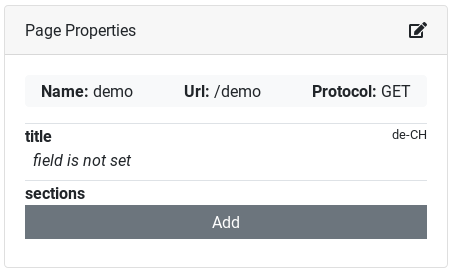
\includegraphics[width=\textwidth]{page_properties.png}
        \caption{View mode.}
        \label{fig.page_properties_view}
    \end{subfigure}
    ~
    \begin{subfigure}[b]{0.49\textwidth}
        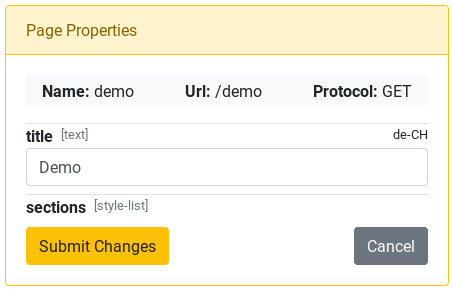
\includegraphics[width=\textwidth]{page_properties_edit.png}
        \caption{Edit mode.}
        \label{fig.page_properties_edit}
    \end{subfigure}
    \caption{The \emph{Page Properties} card.}
    \label{fig.page_properties}
\end{figure}

Adding content to the page is done by creating and adding sections to the page.
This can be done by clicking on the button \textbf{Add} below the field \texttt{sections} in the \emph{Page Properties} card.
This opens the \emph{Add Section} form where the name and the style of the new section can be defined.
The name serves only to let you identify the section at a later point and can be any string.
It is, however, recommended to use a logic structure in naming sections (it is a good idea to include the page name into the section name).
Note that the style is always appended to the section name.
The style defines how the section will look like and what type of content can be assigned to it.
Let's choose the style \texttt{container} which is used as wrapper for other styles to be added to the page.
This helps to manage the spacing at the edges of the page.

The \emph{Add Section} form, as depicted in Figure~\ref{fig.add_section}, has several cards:
The \emph{Add Section} card is all that is needed to create a new section.
However, given that there are quite a few styles to choose from the card \emph{Style Selection Helper} may come in handy.
This card aims to group styles into different categories and provides a very short description of each available style.
The two cards \emph{Select an Unassigned Section} and \emph{Select an Existing Section} allow to choose already existing sections without creating a new one where the former lists sections that are assigned to no parent and the latter lists all user-created sections.

\begin{figure}[ht]
    \centering
    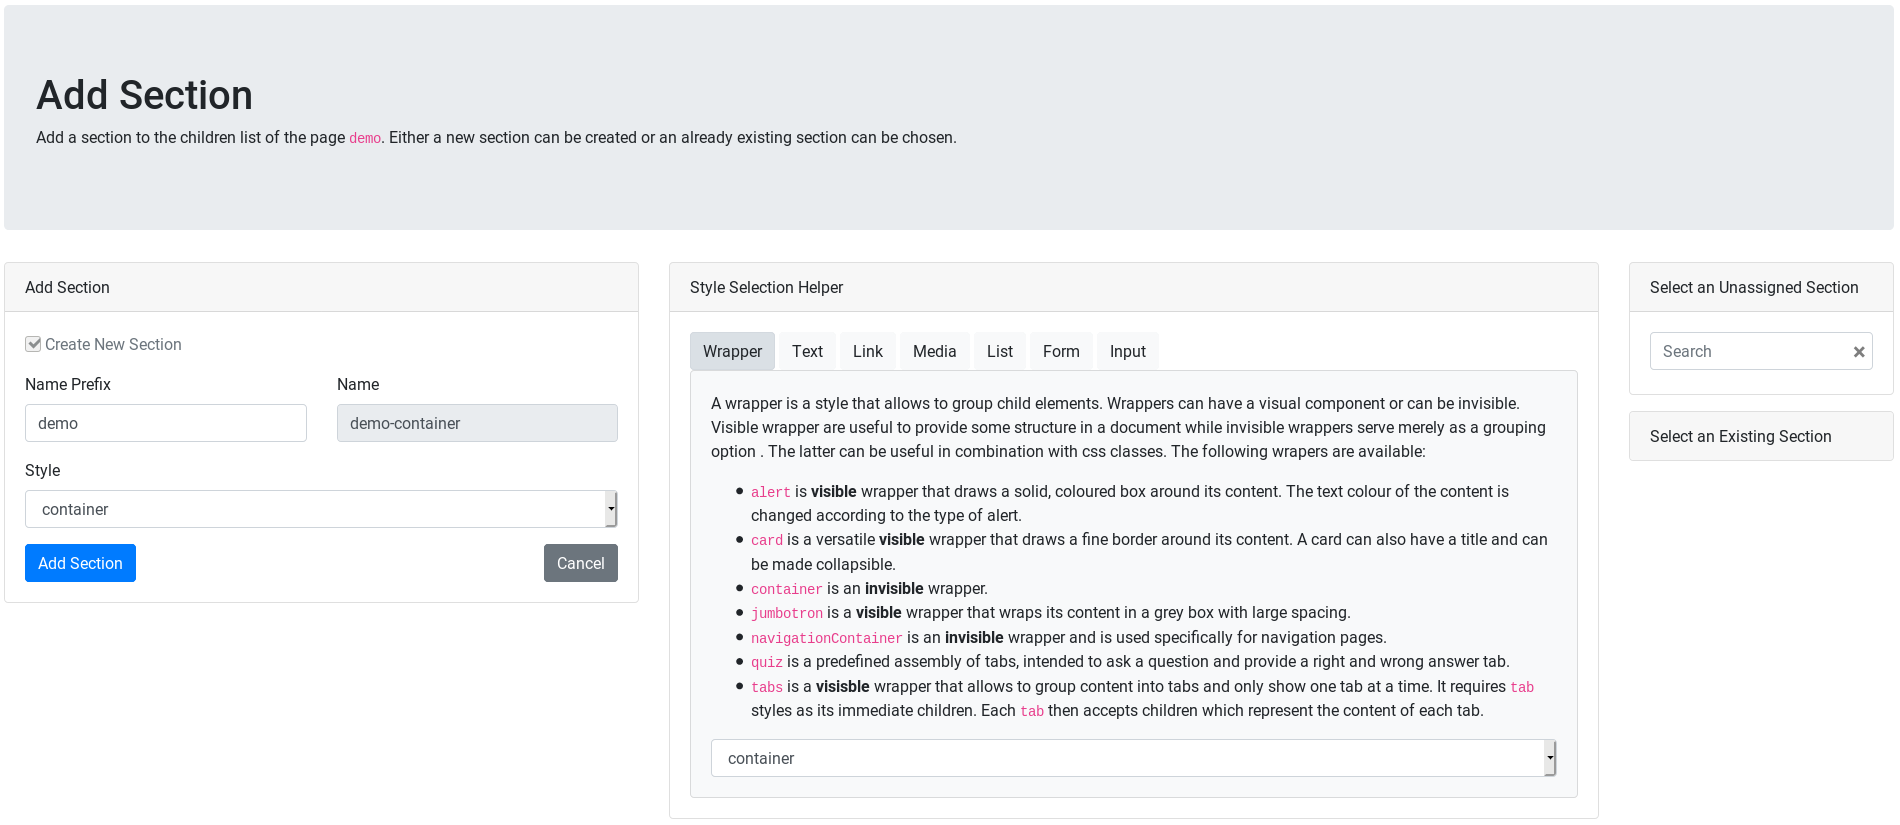
\includegraphics[width=\textwidth]{add_section.png}
    \caption{The \emph{Add Section} form.}
    \label{fig.add_section}
\end{figure}

Click \textbf{Add Section} to create the new section which will return you to the CMS with the new section selected in edit mode (the card \emph{Section Properties} is yellow).

The next step is to edit the properties of the section.
A container section only has the two fields \texttt{CSS} and \texttt{is\_fluid}.
Enable the field \texttt{is\_fluid} to make the container span over the whole page.
The field \texttt{CSS} is special in the sense that every style has this filed.
It allows to specify css classes (sperated by spaces) that will be added to the root html tag of the style.
Add the bootstrap class \Colorbox{light-gray}{\lstinline[columns=fixed]|my-3|} to the field to add some spacing at the top and the bottom of the container (refer to the \href{https://getbootstrap.com/docs/4.1/utilities/spacing/}{Bootstrap documentation} from more details).

Now continue to add sections to the container you just created. For example:
\begin{itemize}
    \item A section of style \texttt{jumbotron} which, itself, holds a section of style \texttt{markdown}.
        In the field \texttt{text\_md} of the markdown section use markdown syntax to add a title and a paragraph of text.
    \item A section of style \texttt{alert} which has a child section of style \texttt{heading} and another child section of style \texttt{plaintext}.
    \item A section of style \texttt{card} which has a child section of style \texttt{quiz}.
\end{itemize}

Doing all of this and tweaking the available fields of the different styles should net you with something resembling Figure \ref{fig.demo}

\begin{figure}[ht]
    \centering
    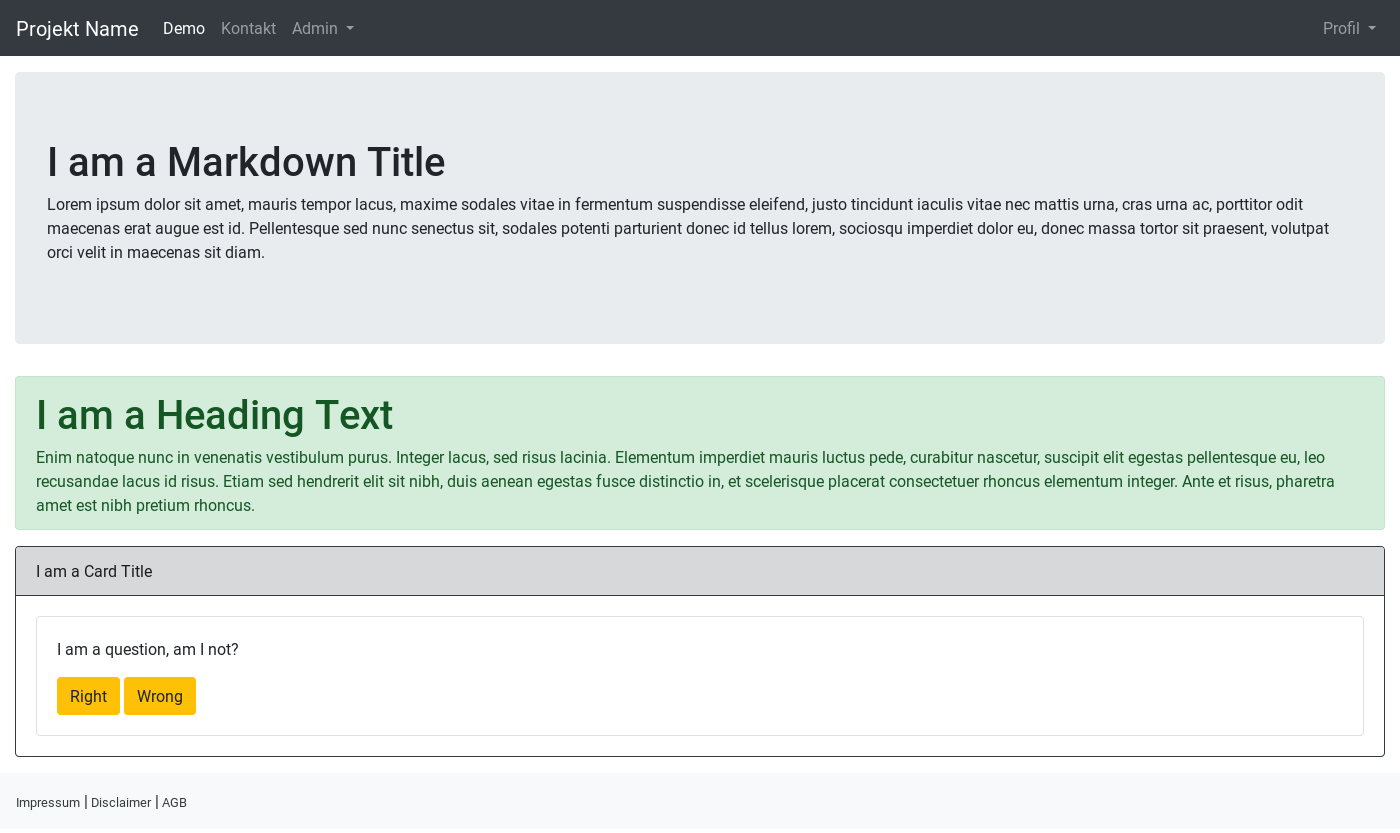
\includegraphics[width=0.95\textwidth]{demo.png}
    \caption{A demo page of type \textbf{Sections}.}
    \label{fig.demo}
\end{figure}

%------------------------------------------------------------------------------
\section{Create a Menu of Pages}
Up to this point we created a section page and added the link to this page to the navigation bar.
It is also possible to create a menu item with multiple page links.
It is, however, not possible to change the position or hierarchy of a page once it is created.
A workaround is to remove the page and create a new one that fits those requirements.
Note that sections remain untouched when a page is deleted, hence, recreating a page with its initial content is not a big deal.

In order to delete a page the \texttt{delete} access right of \textbf{Page Management} is required.
By default users in the group \texttt{admin} and \texttt{experimenter} are granted the mentioned access rights.

As a demonstration let's create a dropdown menu in the navigation bar and add the content we created before as a child element:

First, the recently created page \texttt{demo} has to be removed.
To do this select the page in the \emph{Page Index} of the CMS, open the card \emph{Delete Page} (red), and click the button \textbf{Deplete Page}.
This opens the \emph{Delete Page} from where the keyword of the page has to be entered into the input field to confirm the deleting process.
Click \textbf{Delete Page} and on success click \textbf{Back to CMS} to return to the CMS.

Now, create a new page which will only serve as the root menu item in the navigation bar.
For this purpose I propose to append the string \Colorbox{light-gray}{\lstinline[columns=fixed]|-link|} to the keyword of the new page (e.g \Colorbox{light-gray}{\lstinline[columns=fixed]|demo-link|}).
Enable the field \texttt{Header Position} and choose the appropriate position.
Leave the remaining fields untouched and click \textbf{Create}.

Back in the CMS define the title of the page in the \emph{Page Properties} card as described in the beginning of Section~\ref{sec.add_content}.
Once this is done click the button \textbf{Create New Child Page} in the card \emph{Create New Child Page}.
Once again the \emph{Create New Page} form is opened where we can recreate the page \Colorbox{light-gray}{\lstinline[columns=fixed]|demo|} as described in Section~\ref{sec.new_page} in the beginning of this chapter.
Note that when enabling \texttt{Header Position} only the new page is shown.
This is because this page is the first child page in this menu and the position refers to the current hierarchy level of the page (i.e. to the children of the page \Colorbox{light-gray}{\lstinline[columns=fixed]|demo-link|}).
Back in the CMS define the title of the page and click the button \textbf{Add} below the field \texttt{sections} to add the sections we created before.

Once the \emph{Add Section} form opens you will notice that on the right in the card \emph{Unassigned Sections} the container section we create before is listed.
Select this section and click \textbf{Add Section} which will restore the page as it is represented in Figure \ref{fig.demo} with the exception that now, the page is reachable through a dropdown menu in the navigation bar.

%------------------------------------------------------------------------------
\section{Create a Navigation Page}
Often, it might be interesting to navigate from page to page by clicking on buttons \textbf{Next} and \textbf{Back} or by selecting the corresponding page in a list.
To achieve this the page type \texttt{Navigation} can be used.
A navigation page is a special type of section page where only one immediate child section (which can hold any number of child sections) is rendered at a time.

\begin{figure}[ht]
    \centering
    \begin{subfigure}[t]{0.22\textwidth}
        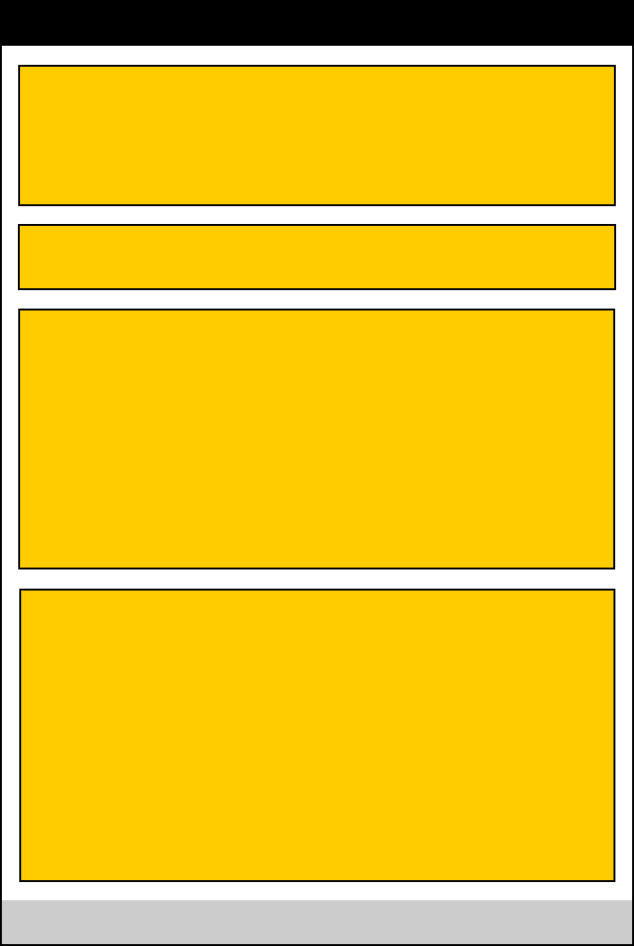
\includegraphics[width=\textwidth]{section_page.png}
        \caption{A section page with four sections.}
        \label{fig.section_page}
    \end{subfigure}
    ~
    \begin{subfigure}[t]{0.22\textwidth}
        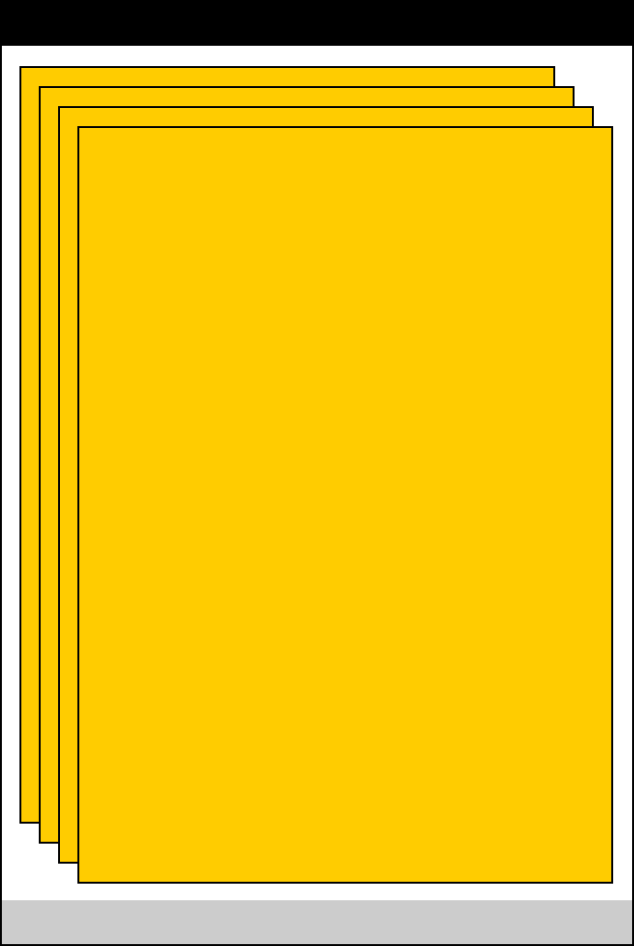
\includegraphics[width=\textwidth]{nav_page.png}
        \caption{A navigation page with four sections (abstract view).}
        \label{fig.nav_page}
    \end{subfigure}
    ~
    \begin{subfigure}[t]{0.22\textwidth}
        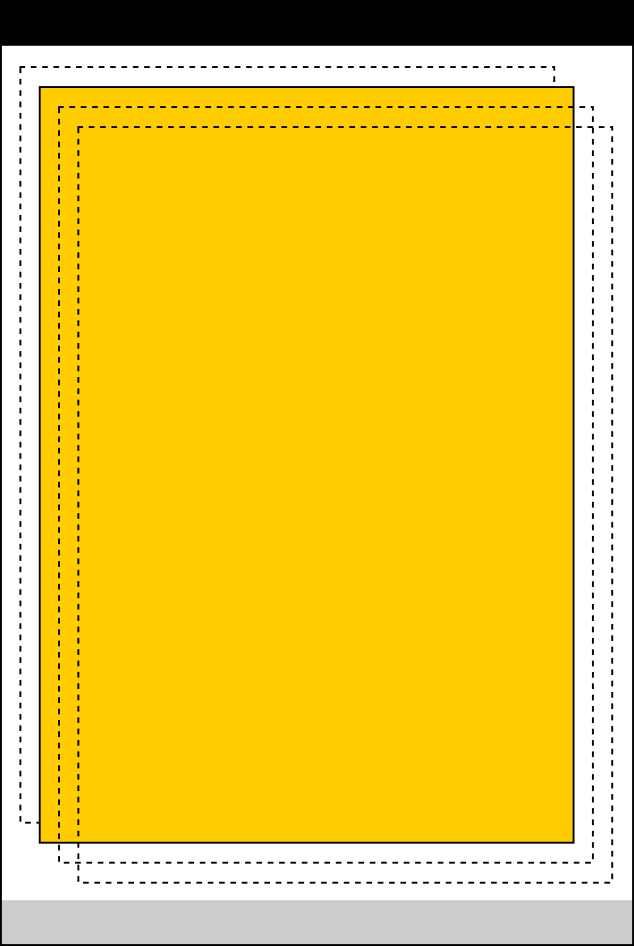
\includegraphics[width=\textwidth]{nav_page_url.png}
        \caption{A navigation page where section $2$ is active.}
        \label{fig.nav_page_url}
    \end{subfigure}
    ~
    \begin{subfigure}[t]{0.22\textwidth}
        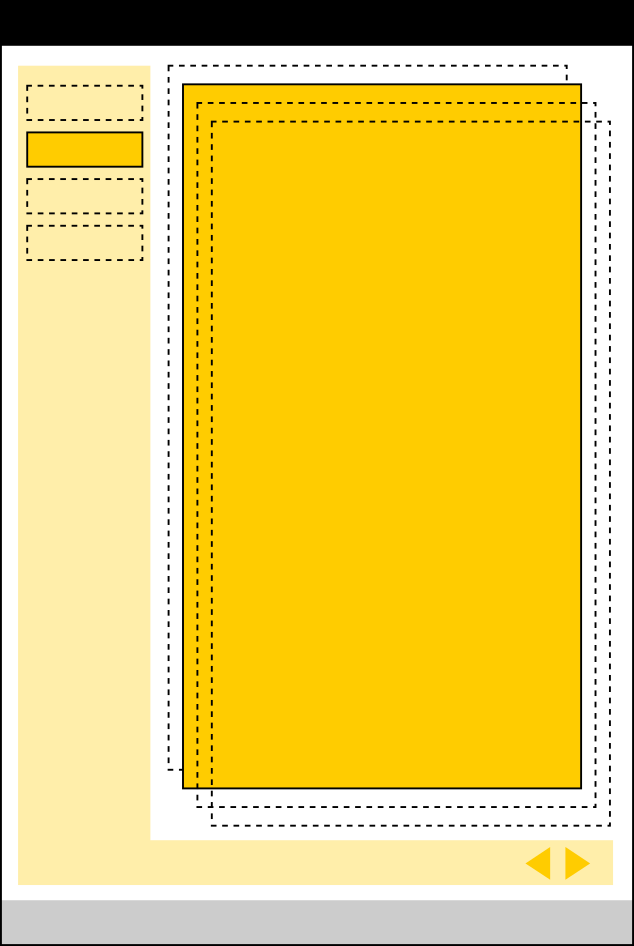
\includegraphics[width=\textwidth]{nav_page_menu.png}
        \caption{A navigation page with control elements to navigate through navigation sections.}
        \label{fig.nav_page_menu}
    \end{subfigure}
    \caption{A conceptual representation of a section page and a navigation page.}
    \label{fig.page_types}
\end{figure}

Figure~\ref{fig.page_types} aims at visualizing this concept.
Figure~\ref{fig.section_page} shows a simple section page with four immediate child sections.
Figure~\ref{fig.nav_page} shows a representation of a navigation page with four immediate child sections.
The sections of the section page are represented one below the other.
However, the sections of the navigation page are represented like they were stacked on top of other like a card deck.
In the following, such sections of a navigation page are called navigation sections.
Note that only one navigation section of a navigation page can be visible.
This is indicated on Figure~\ref{fig.nav_page_url}.
A predefined set of buttons can be rendered on a navigation page which allows to navigate through all navigation sections associated to this page.
Also, a menu can be rendered on a navigation page or any other page which allows to navigate through navigation sections and jump to a specific section.
This is indicated on Figure~\ref{fig.nav_page_menu}.

A navigation page has several characteristics:
\begin{itemize}
    \item A navigation page can only be rendered if the navigation section to be displayed is specified (this is done via the url).
    \item Because of the previous point a navigation page always points to its first entry when displayed as a menu in the header.
    \item A navigation section can only have the style \texttt{navigationContainer}. However, children of such a section can have any style.
\end{itemize}

To demonstrate how a navigation page works, let us create such a page.

We start by creating a new page of type \texttt{Navigation}.
Let this page be a child of the page \Colorbox{light-gray}{\lstinline[columns=fixed]|demo-link|}.
There is no real importance to this but it helps to keep things grouped together in the CMS.
So, select the page \Colorbox{light-gray}{\lstinline[columns=fixed]|demo-link|} and click the button \textbf{Create New Child Page}.
Set a keyword (e.g. \Colorbox{light-gray}{\lstinline[columns=fixed]|demo-nav|}) and set the type to \texttt{Navigation}.
Note that the pattern \Colorbox{light-gray}{\lstinline[columns=fixed]|[i:nav]|} is appended to the \texttt{Url Pattern}.
This pattern will be replaced by the id of the selected navigation section to be displayed on the naviagtion page.

Back in the CMS the page fields can be edited.
As with section pages, the field \texttt{title} defines what will be displayed in the browser tab.
The field \texttt{css\_nav} allows to add css classes to the navigation list that is displayed to the left of a navigation page.
The fields \texttt{label\_back} and \texttt{label\_next} will be the labels of the navigation buttons \textbf{Next} and \textbf{Back}, respectively.
These buttons will only be displayed if the field \texttt{has\_navigation\_buttons} is enabled.
The field \texttt{is\_fluid} defines whether the content is stretched to the whole of the page or not.
For more information about the rest of the available fields refer to the \href{https://selfhelp.psy.unibe.ch/demo/style/362}{\texttt{nestedList} style documentation}.

In order to add a stack of navigation sections to this navigation page the \textbf{Add} button below the field \texttt{navigation} can be used.

Note that a navigation page has a field \texttt{sections} (which we already know from section pages).
This allows to add sections that are rendered before the selected navigation section and will remain the same, independent of the navigation section that is currently displayed (refer to Figure~\ref{fig.demo-nav-page-head} for an example).

Let's add some navigation sections:
Click the \textbf{Add} button below the field \texttt{navigation} which will open the \emph{Add Navigation Section} form.
This is a simplified \emph{Add Section} form where only a name can be chosen.
Note that the style is fixed to \texttt{navigationContainer} and cannot be changed.
Set the name (e.g. \Colorbox{light-gray}{\lstinline[columns=fixed]|demo-nav1|}) and click \textbf{Add Section} to complete the process.
In the Section Properties card, the field \texttt{title} serves as title for the navigation list item representing the navigation section wrapped by this container.
The field \texttt{text\_md} is rendered at the top of the navigation section.
Note that the special string \Colorbox{light-gray}{\lstinline[columns=fixed]|@title|} can be used to render the field \texttt{title} within the field \texttt{text\_md}.
Finally, the field \texttt{CSS} allows to add css classes to the navigation container section to modify its visual aspects.

As an example set the field \texttt{title} to \Colorbox{light-gray}{\lstinline[columns=fixed]|Nav 1|} and the field \texttt{text\_md} to \Colorbox{light-gray}{\lstinline[columns=fixed]|# Demo @title|} (the \# symbol is markdown syntax for a heading of level 1) and click \textbf{Submit Changes}.

In order to truly see how navigation pages work we have to add some more navigation sections.
Do this by selecting the page \Colorbox{light-gray}{\lstinline[columns=fixed]|demo-nav|} and adding two more navigation sections with the titles \Colorbox{light-gray}{\lstinline[columns=fixed]|Nav 2|} and \Colorbox{light-gray}{\lstinline[columns=fixed]|Nav 3|}.

\subsection{Linking to Navigation Sections}
Up to this point we created a navigation page with three navigation sections but have currently no way of accessing them.
As noted before, in order to display a navigation page an id of a navigation section needs to be specified in the url.
Let's assume that the keyword of the navigation page is \Colorbox{light-gray}{\lstinline[columns=fixed]|demo-nav|}, the base path of the WebApp is \Colorbox{light-gray}{\lstinline[columns=fixed]|https://selfhelp.psy.unibe.ch/myapp|}, and the id of the navigation section we want to display is \Colorbox{light-gray}{\lstinline[columns=fixed]|n|} (Note that the id of a section is the last number in the url when selecting this section in the CMS).
The url to access this navigation section would then be \Colorbox{light-gray}{\lstinline[columns=fixed]|https://selfhelp.psy.unibe.ch/myapp/demo-nav/n|}.

Obviously, it is rather cumbersome to reach a navigation page this way which is why there is a mechanism to automatically generate these links.
There exist three possibilities to generate links to a navigation section:
\begin{enumerate}
    \item When checking the \emph{Header Position} during the page creation step of a navigation page a link is generated which points to the first navigation section of the navigation page.
    \item When using a link style (e.g. styles \texttt{link} or \texttt{button}), the field \texttt{url} can be set to a pattern of the specific form
        \Colorbox{light-gray}{\lstinline[columns=fixed]|#<nav_page>/<nav_section>|} where \Colorbox{light-gray}{\lstinline[columns=fixed]|<nav\_page>|} is the keyword of the navigation page and \Colorbox{light-gray}{\lstinline[columns=fixed]|<nav\_section>|} the name of the navigation section.
        E.g. assuming that the navigation page keyword is \Colorbox{light-gray}{\lstinline[columns=fixed]|demo-nav|} and the navigation section has the name \Colorbox{light-gray}{\lstinline[columns=fixed]|demo-nav1-navigationContainer|}, to access the navigation section the field \texttt{url} would be set to \Colorbox{light-gray}{\lstinline[columns=fixed]|#demo-nav/demo-nav1-navigationContainer|}.
    \item A list style \texttt{nestedList} allows to be linked to a navigation page which will automatically generate the list of all navigation sections attributed to the navigation page.
        This is accomplished by setting the field \texttt{items} to the pattern \Colorbox{light-gray}{\lstinline[columns=fixed]|{"nav_page": "<nav_page>"}|} where \Colorbox{light-gray}{\lstinline[columns=fixed]|<nav_page>|} is the keyword of the navigation page to be linked.
        E.g. assuming that the navigation page keyword is \Colorbox{light-gray}{\lstinline[columns=fixed]|demo-nav|}, to generate the list of links to all navigation sections the field \texttt{items} would be set to \Colorbox{light-gray}{\lstinline[columns=fixed]|{"nav_page": "demo-nav"}|}.
\end{enumerate}

To demonstrate how to link the navigation page \Colorbox{light-gray}{\lstinline[columns=fixed]|demo-nav|} and all its navigation sections, let's use a nested list:
We can achieve this by adding a new section to the page \Colorbox{light-gray}{\lstinline[columns=fixed]|demo|} we created in the beginning.
Select the page \Colorbox{light-gray}{\lstinline[columns=fixed]|demo|} and add a new child section of style \texttt{nestedList} to the page:
\begin{enumerate}
    \item Select any container section or the page itself and click \textbf{Add} below the field \texttt{children} or \texttt{sections}, respecively.
    \item Select the style \texttt{nestedList} (from style group \texttt{List}).
    \item Enter a name (e.g. \Colorbox{light-gray}{\lstinline[columns=fixed]|demo-nav-link|}).
    \item Click \textbf{Add Section}.
    \item In the card \emph{Section Properties} fill out the field \texttt{items} with the content \Colorbox{light-gray}{\lstinline[columns=fixed]|{"nav_page": "demo-nav"}|}.
        This is a special \href{http://www.json.org/}{json} string which tells the nested list to go and fetch all navigation sections of the navigation page \Colorbox{light-gray}{\lstinline[columns=fixed]|demo-nav|}.
    \item Leave everything else as is and click \textbf{Submit Changes}.
\end{enumerate}

As a result you should get something similar to what is represented in Figure \ref{fig.demo-nav}.

\begin{figure}[ht]
    \centering
    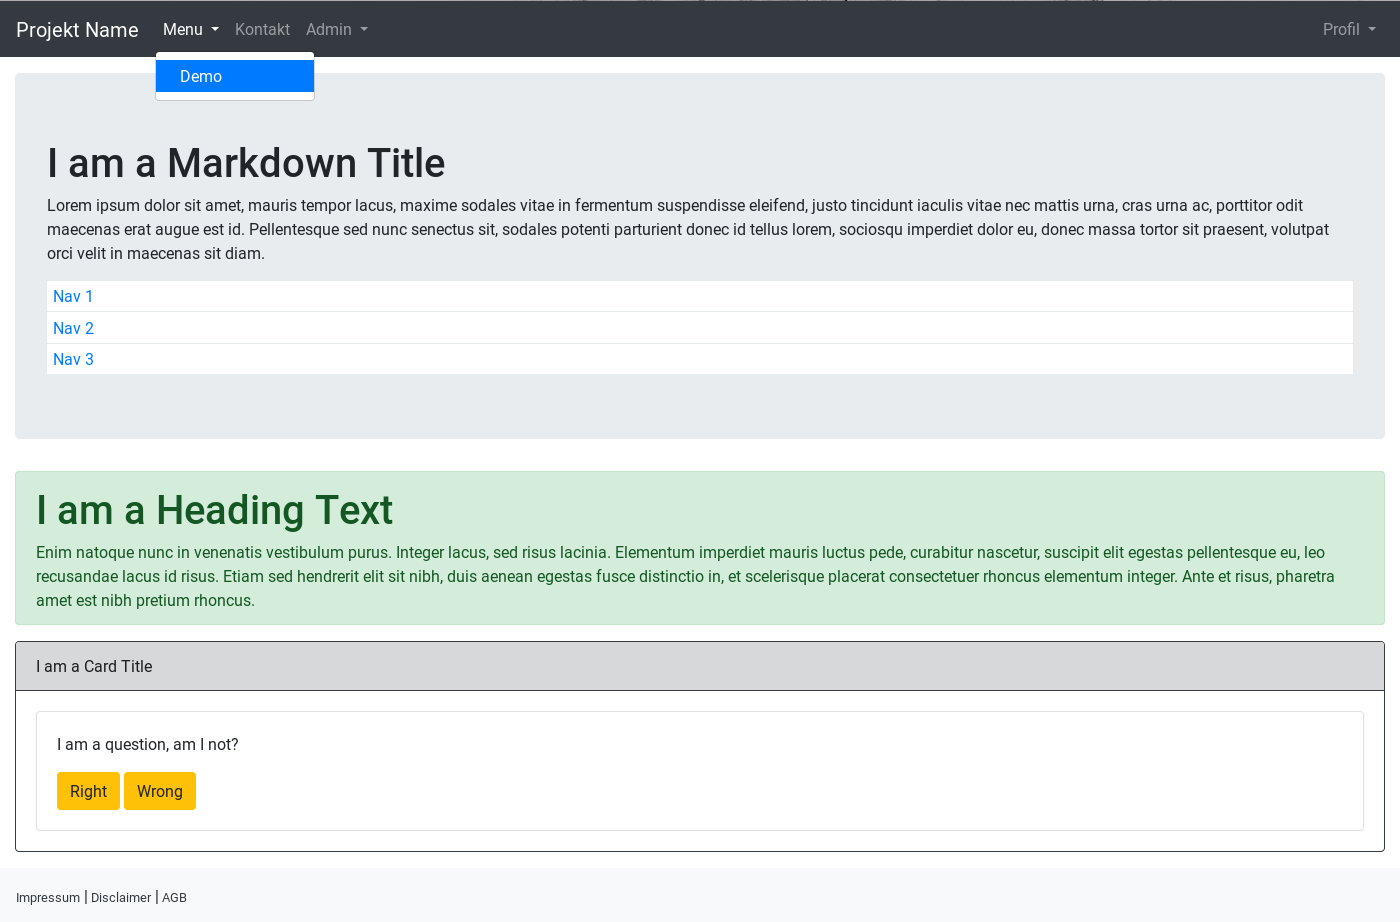
\includegraphics[width=0.95\textwidth]{demo-nav.png}
    \caption{A demo page of type \textbf{Sections} with a list of navigation items added to the jumbatron.}
    \label{fig.demo-nav}
\end{figure}

The navigation page \Colorbox{light-gray}{\lstinline[columns=fixed]|demo-nav|} is reached by clicking on any of the items displayed in the nested list.
The result should look similar to Figure \ref{fig.demo-nav-page}.

\begin{figure}[ht]
    \centering
    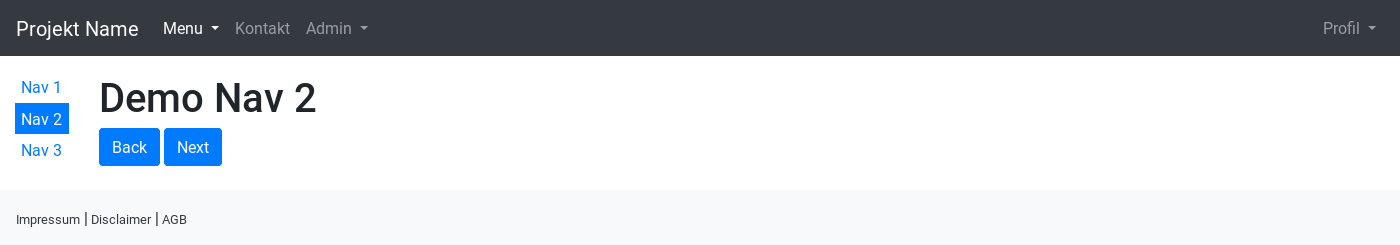
\includegraphics[width=0.95\textwidth]{demo-nav-page.png}
    \caption{A demo page of type \textbf{Navigation} with a list of navigation items displayed on the left and navigation buttons displayed at the bottom of the page.}
    \label{fig.demo-nav-page}
\end{figure}

Note that sections that are added to the navigation page \Colorbox{light-gray}{\lstinline[columns=fixed]|demo-nav|} through the filed \texttt{sections} will appear on top of each navigation section as demonstrated in Figure \ref{fig.demo-nav-page-head}.

\begin{figure}[ht]
    \centering
    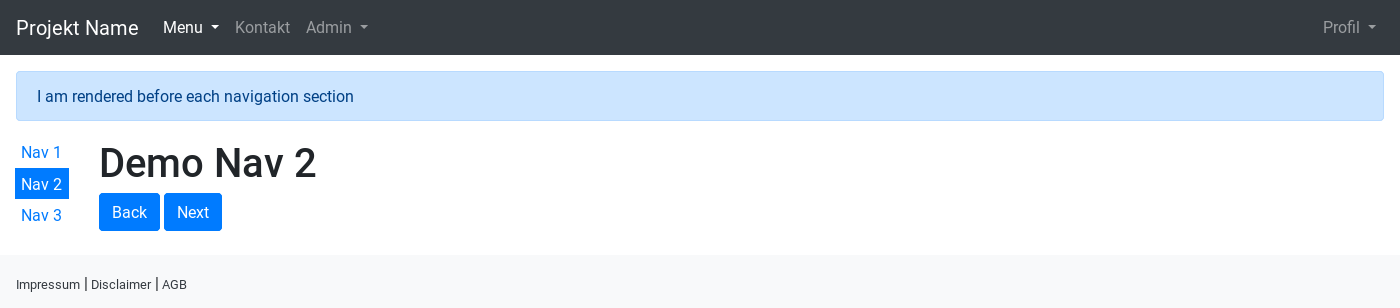
\includegraphics[width=0.95\textwidth]{demo-nav-page-head.png}
    \caption{A demo page of type \textbf{Navigation} where before each navigation section the same section is displayed (the blue alert box).}
    \label{fig.demo-nav-page-head}
\end{figure}

Also note that navigation sections can be arranged hierarchically by using the field \texttt{navigation} in the card \emph{Section Properties} of a navigation section and adding a child navigation section.

%==============================================================================
\chapter{Symbols with Special Meaning}
In order to facilitate the usage of certain styles several keywords can be used to render user-specific data, easily link to pages, or refer to stored files.
The following list provides an overview of all available keywords in the different styles:

\begin{itemize}
    \item In any field of any style the following keywords can be used:
        \begin{description}
            \item[\textbf{\texttt{@user}}] This keyword is replaced with the name the user provided during the validation process.
            \item[\textbf{\texttt{@project}}] This keyword is replaced with the title of the page \texttt{home}.
        \end{description}
    \item In the styles \texttt{form}, \texttt{link} and \texttt{button} links can be generated if a special syntax is used:
        \begin{description}
            \item[\textbf{\texttt{\#self}}] refers to the current page.
            \item[\textbf{\texttt{\#back}}] refers to the page that was visited previously.
                Note that if the previous page cannot be found \texttt{\#back} is equivalent to \texttt{\#home}.
            \item[\textbf{\texttt{\%<asset\_name>}}] links to a asset where \Colorbox{light-gray}{\lstinline[columns=fixed]|<asset_name>|} is the exact name of the asset.
            \item[\textbf{\texttt{\#<page\_name>}}] links to a page where \Colorbox{light-gray}{\lstinline[columns=fixed]|<page_name>|} is the keyword of the page.
            \item[\textbf{\texttt{\#<page\_name>\#<wrapper\_name>}}] links to an anchor on a page where \Colorbox{light-gray}{\lstinline[columns=fixed]|<page_name>|} is the keyword of the page and \Colorbox{light-gray}{\lstinline[columns=fixed]|<wrapper_name>|} is the name of a section that is used as an anchor.
                Note that the anchor section must be of one of the following styles for this to work: \texttt{alert}, \texttt{container}, \texttt{card}, \texttt{form}.
            \item[\textbf{\texttt{\#<nav\_page\_name>/<section\_name>}}] links to a navigation section on a navigation page where \Colorbox{light-gray}{\lstinline[columns=fixed]|<nav_page_name>|} is the keyword of the navigation page and \Colorbox{light-gray}{\lstinline[columns=fixed]|<section_name>|} is the name of the navigation section.
            \item[\textbf{\texttt{\#<page\_name>/<section\_name>\#<wrapper\_name>}}] links to an anchor on a navigation section on a navigation page where \Colorbox{light-gray}{\lstinline[columns=fixed]|<nav_page_name>|} is the keyword of the navigation page, \Colorbox{light-gray}{\lstinline[columns=fixed]|<section_name>|} is the name of a navigation section, and \Colorbox{light-gray}{\lstinline[columns=fixed]|<wrapper_name>|} is the name of a section that is used as anchor.
                Note that the anchor section must be of one of the following styles for this to work: \texttt{alert}, \texttt{container}, \texttt{card}, \texttt{form}.
        \end{description}
    \item The field \texttt{text\_md} of the style \texttt{navigationContainer} allows the keyword \Colorbox{light-gray}{\lstinline[columns=fixed]|@title|} to refer to the field \texttt{title} of the navigation container.
    \item The field \texttt{condition} of style \texttt{conditionalContainer} allows the keyword \Colorbox{light-gray}{\lstinline[columns=fixed]|@<form_name>#<field_name>|} to refer to the user data of a specific input field \Colorbox{light-gray}{\lstinline[columns=fixed]|<field_name>|} of a specific form \Colorbox{light-gray}{\lstinline[columns=fixed]|<form_name>|}.
\end{itemize}

%==============================================================================
\chapter{User Input}\label{sec.user_input}

The SelfHelp WebApp provides several styles to work with user input.
The style \texttt{formUserInput} can be used to store data, entered by a user, to the database.
The style \texttt{showUserInput} is a simple style that allows top display data that was entered by a user via a specific section of style \texttt{formUserInput}.
Finally, the style \texttt{conditionalContainer} allows to evaluate user input and display content depending on the outcome of the evaluation.

\section{Store User Data to the Database}
The Selfhelp WebApp allows to create html forms where user input is automatically stored to the database.
In order for a page to be allowed to send data to the server the following two conditions need to be met:
\begin{enumerate}
    \item The \texttt{POST} protocol needs to be enabled when creating a new page.
        This is enabled by default.
        The protocol of a page is set when creating a new page (advanced options).
    \item The page requires input fields, wrapped by a form such that users can enter and submit their data.
        Forms and their input fields are added to a page by adding sections with styles from the groups \texttt{Form} and \texttt{Input}, respectively.
\end{enumerate}

There are two ways of how user data is stored to the database automatically:
\begin{enumerate}
    \item Data is continuously updated.
        In this case an input field always shows the current, user-specific content and whenever this content is changed by the user, the old values are overwritten in the database.
        This way of storing data is intended for entries where data is constantly edited and revised.
    \item Data is stored incrementally.
        In this case each time a set of data is submitted to the server, a timestamp is attached to the data.
        For each submission a new entry is created in the database which allows to store multiple entries, made at different points in time.
        This way of storing the data is intended for log-like forms where a user is asked to enter a specific set of data every day.
\end{enumerate}

As a demonstration let's add a new section page (set \emph{Page Type} to \texttt{Sections}) with keyword \Colorbox{light-gray}{\lstinline[columns=fixed]|user_input|} and title \Colorbox{light-gray}{\lstinline[columns=fixed]|User Input|} to the demo application.
Remember to check the \emph{User Input} checkbox (in order to allow user input) and the \emph{Header Position} checkbox (to place the page in the header) in the \emph{Create New Page} form.

Next, add sections to this page to get a similar result as represented in Figure~\ref{fig.form-empty}.
This is accomplished by adding the following sections hierarchically to the page \Colorbox{light-gray}{\lstinline[columns=fixed]|user_input|}:
\begin{itemize}
    \item a \texttt{container} with \texttt{css} $=$ \Colorbox{light-gray}{\lstinline[columns=fixed]|my-3|} and \texttt{is\_fluid} enabled
        \begin{itemize}
            \item a \texttt{card} with \texttt{title} $=$ \Colorbox{light-gray}{\lstinline[columns=fixed]|Diary|}
                \begin{itemize}
                    \item a \texttt{formUserInput} with \texttt{name} $=$ \Colorbox{light-gray}{\lstinline[columns=fixed]|diary|}, \texttt{alert\_success} $=$ \Colorbox{light-gray}{\lstinline[columns=fixed]|Well done|}, and \texttt{label} $=$ \Colorbox{light-gray}{\lstinline[columns=fixed]|Submit|}
                        \begin{itemize}
                            \item a \texttt{textarea} with \texttt{name} $=$ \Colorbox{light-gray}{\lstinline[columns=fixed]|diary-thought|} and \texttt{label} $=$ \Colorbox{light-gray}{\lstinline[columns=fixed]|My Thoughts|}
                            \item a \texttt{textarea} with \texttt{name} $=$ \Colorbox{light-gray}{\lstinline[columns=fixed]|diary-action|} and \texttt{label} $=$ \Colorbox{light-gray}{\lstinline[columns=fixed]|My Actions|}
                        \end{itemize}
                \end{itemize}
            \item a \texttt{card} with \texttt{title} \Colorbox{light-gray}{\lstinline[columns=fixed]|Log|} and \texttt{css} $=$ \Colorbox{light-gray}{\lstinline[columns=fixed]|mt-3|}
                \begin{itemize}
                    \item a \texttt{formUserInput} with \texttt{name} $=$ \Colorbox{light-gray}{\lstinline[columns=fixed]|log|}, \texttt{alert\_success} $=$ \Colorbox{light-gray}{\lstinline[columns=fixed]|Well done|}, \texttt{label} $=$ \Colorbox{light-gray}{\lstinline[columns=fixed]|Submit|}, and with \texttt{is\_log} checked
                        \begin{itemize}
                            \item an \texttt{input} with \texttt{type\_input} $=$ \Colorbox{light-gray}{\lstinline[columns=fixed]|time|}, \texttt{name} $=$ \Colorbox{light-gray}{\lstinline[columns=fixed]|log-alarm|}, and \texttt{label} $=$ \Colorbox{light-gray}{\lstinline[columns=fixed]|Set my Alarm to|}
                            \item an \texttt{input} with \texttt{type\_input} $=$ \Colorbox{light-gray}{\lstinline[columns=fixed]|time|}, \texttt{name} $=$ \Colorbox{light-gray}{\lstinline[columns=fixed]|log-up|}, and \texttt{label} $=$ \Colorbox{light-gray}{\lstinline[columns=fixed]|Stood up at|}
                            \item an \texttt{input} with \texttt{type\_input} $=$ \Colorbox{light-gray}{\lstinline[columns=fixed]|text|}, \texttt{name} $=$ \Colorbox{light-gray}{\lstinline[columns=fixed]|log-word|}, \texttt{label} $=$ \Colorbox{light-gray}{\lstinline[columns=fixed]|First Word of the Day|}, and \texttt{placeholder} $=$ \Colorbox{light-gray}{\lstinline[columns=fixed]|What did you think when you heard the Alarm|}
                        \end{itemize}
                \end{itemize}
        \end{itemize}
\end{itemize}

Note that when entering and submitting data in the form in card \Colorbox{light-gray}{\lstinline[columns=fixed]|Diary|} the data persists in the input fields even when refreshing the page.
By changing the data and resubmitting, the database entry on the server is overwritten with the new content.
In contrast to this, when entering and submitting data in the form in card \Colorbox{light-gray}{\lstinline[columns=fixed]|Log|} the data disappears and the input fields are set back to its default value.
In this second case the data is stored incrementally in the database and is not fed back to the input fields.

This difference is configured by checking (store incrementally) or unchecking (update in place) the \texttt{is\_log} field of the style \texttt{formUserInput}.

\begin{figure}[ht]
    \centering
    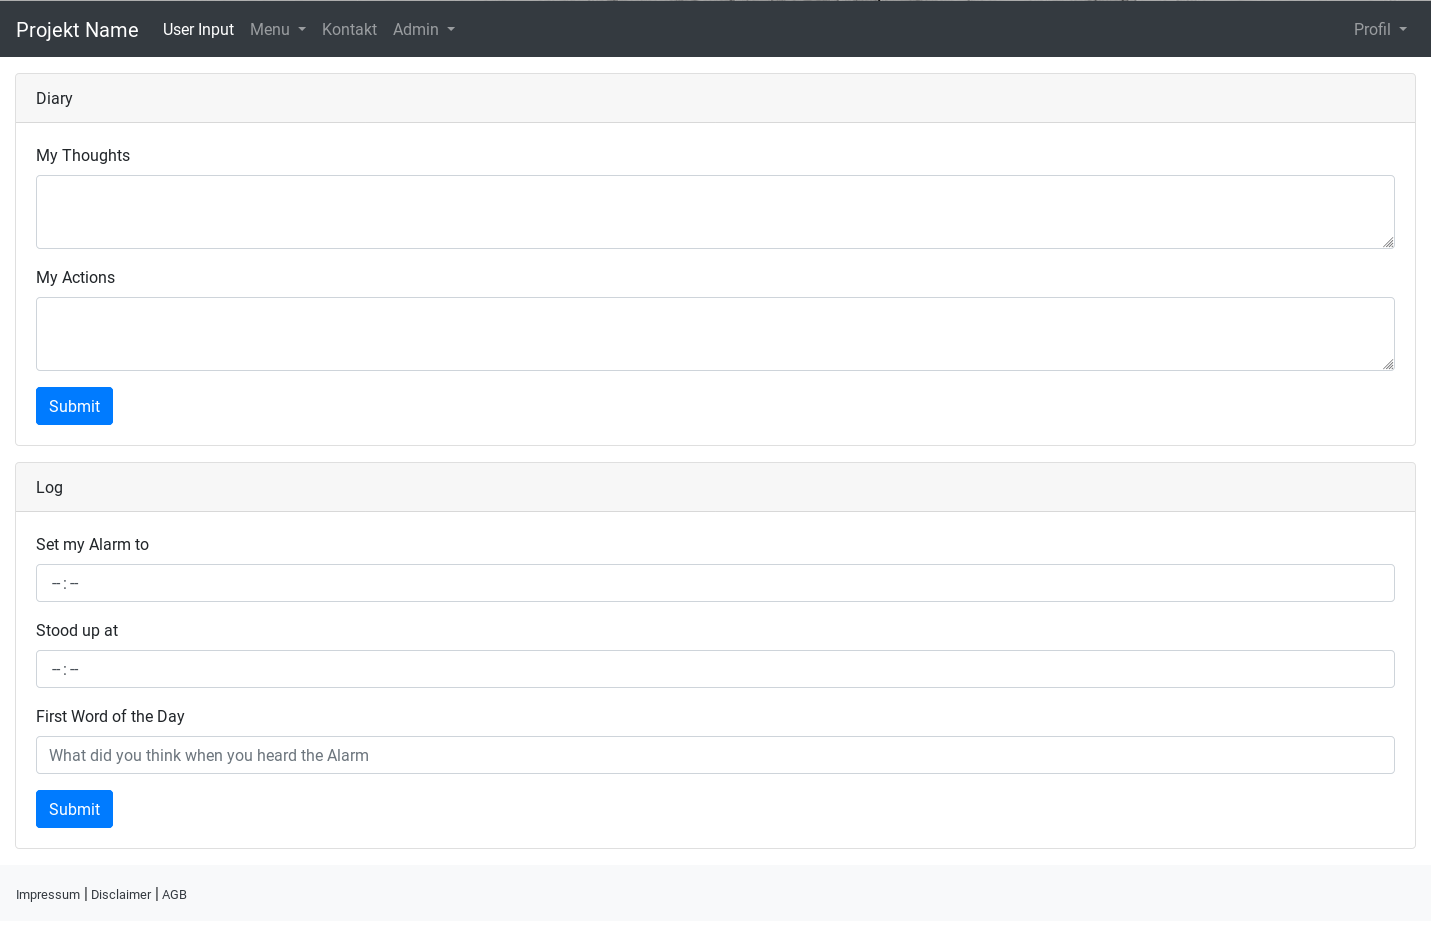
\includegraphics[width=0.95\textwidth]{form_empty.png}
    \caption{A demo page with user input fields and submit buttons to send the data to the server.}
    \label{fig.form-empty}
\end{figure}

\section{Fetch User Data from the Database}

In order to fetch user input and display it on the screen the style \texttt{showUserInput} can be used.
All that needs to be done is creating a section with style \texttt{showUserInput} and set the field \texttt{source} to the \texttt{name} of the form from which the data should be displayed.

As a demonstration let's add a new section page (set \emph{Page Type} to \texttt{Sections}) with keyword \Colorbox{light-gray}{\lstinline[columns=fixed]|show_user_input|} and title \Colorbox{light-gray}{\lstinline[columns=fixed]|Show User Input|} to the demo application.
Remember to check the \emph{Header Position} checkbox (to place the page in the header) in the \emph{Create New Page} form.

Next, add the following sections hierarchically to the page \Colorbox{light-gray}{\lstinline[columns=fixed]|show_user_input|}:
\begin{itemize}
    \item a \texttt{container} with \texttt{css} $=$ \Colorbox{light-gray}{\lstinline[columns=fixed]|my-3|}
        \begin{itemize}
            \item a \texttt{card} with \texttt{title} $=$ \Colorbox{light-gray}{\lstinline[columns=fixed]|Show Diary|}
                \begin{itemize}
                    \item a \texttt{showUserInput} with \texttt{source} $=$ \Colorbox{light-gray}{\lstinline[columns=fixed]|diary|}
                \end{itemize}
            \item a \texttt{card} with \texttt{title} \Colorbox{light-gray}{\lstinline[columns=fixed]|Show Log|} and \texttt{css} $=$ \Colorbox{light-gray}{\lstinline[columns=fixed]|mt-3|}
                \begin{itemize}
                    \item a \texttt{showUserInput} with \texttt{source} $=$ \Colorbox{light-gray}{\lstinline[columns=fixed]|log|}, \texttt{label\_date\_time} $=$ \Colorbox{light-gray}{\lstinline[columns=fixed]|Date|}, and with \texttt{is\_log} checked
                \end{itemize}
        \end{itemize}
\end{itemize}

Note that if the field \texttt{is\_log} of the style \texttt{showUserInput} is set the data items are displayed as a table with a timestamp column and the input field names as column titles.
However if \texttt{is\_log} is not set the timestamp disappears and the input field names are used as row headings.

If instead of the style \texttt{formUserInput} the style \texttt{form} is used, the input data is not automatically stored in the database.
In this case a custom style or component needs to be created which is handling the user data (see Chapter~\ref{sec.extend}).

\section{Conditional Content}
Sometimes it might be interesting to display data depending on an input provided by the user.
Such a behaviour can be achieved with the help of the style \texttt{conditionalContainer}.
A section of this style simply wraps its content in a invisible container.
Further, a condition can be attached to such a section which defines whether the content will be displayed or not.
This condition is defined in the field \texttt{condition} of the style.
Defining a condition might be a bit tricky when first encountering it because it is based on a \href{http://www.json.org/}{json} syntax and requires a bit of getting used to.
It is, however, rather flexible and might be replaced with a more intuitive interface in the future.

For detailed information about the syntax for the condition field refer to the \href{https://selfhelp.psy.unibe.ch/demo/style/446}{\texttt{conditionalContainer} style documentation}.

%==============================================================================
\chapter{User Management}\label{sec.user}
In order to view, create, modify, and delete users and groups the \texttt{select}, \texttt{insert}, \texttt{update}, and \texttt{delete} access rights of \textbf{User Management} is required.
By default users in the group \texttt{admin} are granted all access rights while the users in the group \texttt{experimenter} are granted all access rights safe \texttt{delete}.

\section{Users}
To manage users navigate to \emph{Users} in the menu \emph{Admin}.
All registered users are listed in a card on the left.
A user can be either \texttt{active} (can log in and visit all accessible pages), \texttt{inactive} (cannot login as long as the account is not verified), or \texttt{blocked} (cannot login until the blocked status is reversed).
The cards on the left hand side provide an interfaces to block, unblock, or delete a user and allow to manage the groups a user belongs to.
A user inherits all access rights of the groups the user belongs to.

\section{Groups}
To manage groups navigate to \emph{Groups} in the menu \emph{Admin}.
All groups are listed in a card on the left.
Manage the access right of each group by checking or unchecking the appropriate checkbox in the card \emph{Group Access Rights}.

\section{Registration of Users}
There are two possibilities to register users:

\begin{enumerate}
    \item Each user is manually created via the menu \emph{Admin/Users} by clicking on the button create new user.
    \item A user can register himself/herself in the registration form by entering a valid email address and a validation code.
\end{enumerate}


%==============================================================================
\chapter{Extending the WebApp}\label{sec.extend}
The code base is designed in a modular way such that it is easy to extend the functionality of a WebApp.
Please refer to the documentation on the \href{https://selfhelp.psy.unibe.ch/demo/extend}{demo page}\footnote{https://selfhelp.psy.unibe.ch/demo/extend} for more information on extending the source code:

\begin{description}
    \item[\href{https://selfhelp.psy.unibe.ch/demo/extend/432}{Workflow}] provides a short overview on how to manage the source code and how to report back the changes made.
    \item[\href{https://selfhelp.psy.unibe.ch/demo/extend/416}{The Concept Behind the Code}] provides an overview on the code structure and introduces the vocabulary used within the code.
    \item[\href{https://selfhelp.psy.unibe.ch/demo/extend/417}{Evaluate User Input}] explains in very broad terms how user inputs can be handled programmatically.
    \item[\href{https://selfhelp.psy.unibe.ch/demo/extend/419}{Customize the Theme}] provides several approaches to change the look and feel of the web app without changing too much of the source code.
    \item[\href{https://selfhelp.psy.unibe.ch/demo/extend/418}{Create a Custom Style}] provides a list of steps to be performed in order to create a custom style.
    \item[\href{https://selfhelp.psy.unibe.ch/demo/extend/420}{Create a Custom Component}] provides a list of steps to be performed in order to create a custom component.
    \item[\href{https://selfhelp.psy.unibe.ch/demo/extend/421}{Create a Custom Page}] provides some hints and guidelines to create a custom page.
\end{description}

\end{document}
